\chapter{Results} \label{chapResults}
\section{Photogrametry on Drone Forest Images}
An important first step in multiple approaches the approaches we used is understanding the structure of the forest scene. We ran Agisoft Metashape with the parameters from \cite{Young2022} on a variety of datasets. Three collects shown in Figure \ref{fig:results:sfm} are representative of the types of we data experimented with. The first dataset, \textit{Stowe}, was collected with a lawnmower survey from a commodity drone. The locations of all the cameras were properly estimated and the results look good throughout. Some geometry of the trees can be seen, but much of the fine detail is lost, which is common for photogrametery. The next collect is \textit{Warton}, which was collected with the custom payload at an off-nadir angle and manual flight pattern observing roughly the same region from different angles. All of the cameras were properly aligned, but the quality of the mesh varies dramatically. In the center where there are multiple observations, the results are fairly good. However, both the structure and texture become more blurry farther away from the central area. This is likely because there are fewer camera view to triangulate and those regions are farther away. This mesh is darker than the \textit{Stowe} it was underexposed, due to a fixed exposure between collects. It is important to balance under- and over-exposure, espectially in regions with different brighnesses. A further consideration is that longer exposures are more prone to motion blur, which is especially common while the drone is turning.
Finally, \textit{Coimbra} is a collect where the drone follows a path between trees. The data is captured with the custom payload facing forward at an off-nadir angle. A large portion of this trajectory appeared to be roughly accurate. However, in multiple instances, a set of cameras and the associated mesh were rotated relative to the correct orientation. This resulted in odd artifacts that made the mesh effectively unusable. Furthermore, the level of visual detail was fairly low.

These results support the common practice of automated drone surveys, since this method yielded consistently high-quality results across all the datasets we experimented on. However, it also shows that manual flight patterns over canopy yield some useful data and challenging under-canopy conditions are somewhat successful. This suggests that traditional drone surveys are well-motivated, but further research on photogrametry for more challenging forest scenarious may yeild useful results.


\begin{figure}[h]
    \subfloat{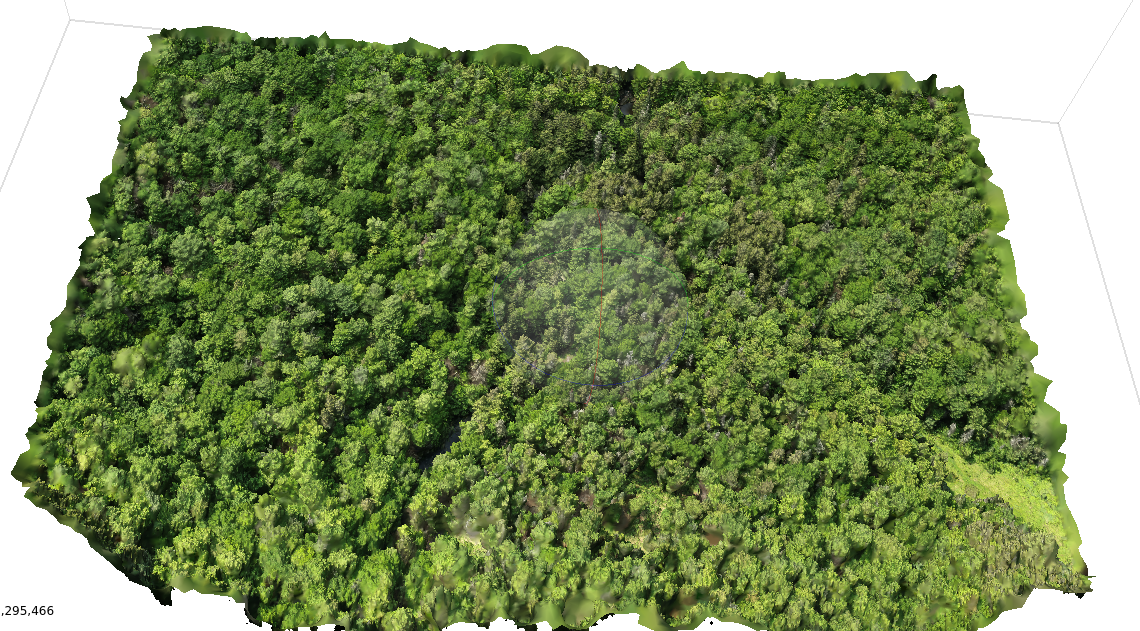
\includegraphics[width=0.45\textwidth]{figs/results/geometric_understanding/stowe_anew_collect_000_zoomed_out.png}}
    \hfill
    \subfloat{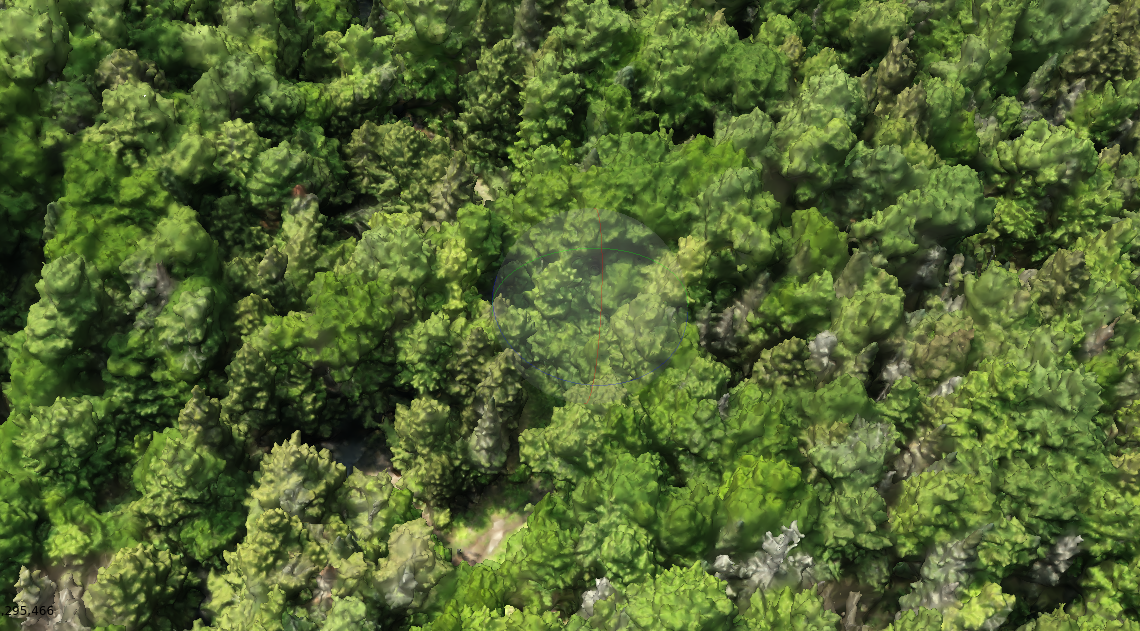
\includegraphics[width=0.45\textwidth]{figs/results/geometric_understanding/stow_anew_collect_000_zoomed_in.png}}\\
        
    \subfloat{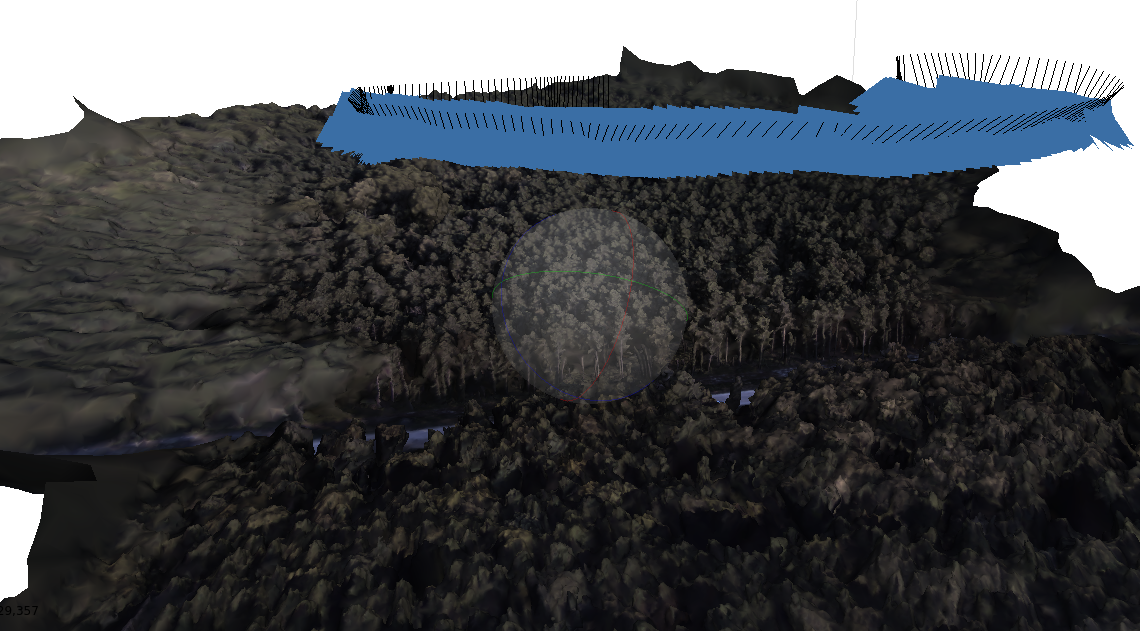
\includegraphics[width=0.45\textwidth]{figs/results/geometric_understanding/burn_zoomed_out.png}}
    \hfill
    \subfloat{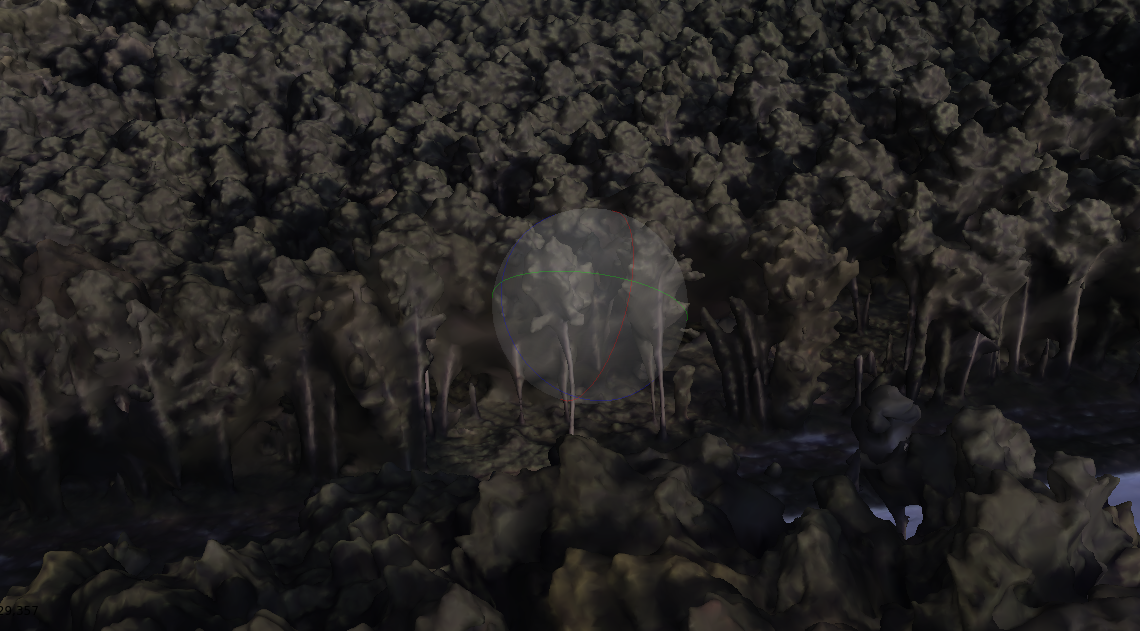
\includegraphics[width=0.45\textwidth]{figs/results/geometric_understanding/burn_zoomed_in.png}}\\
    
    \subfloat{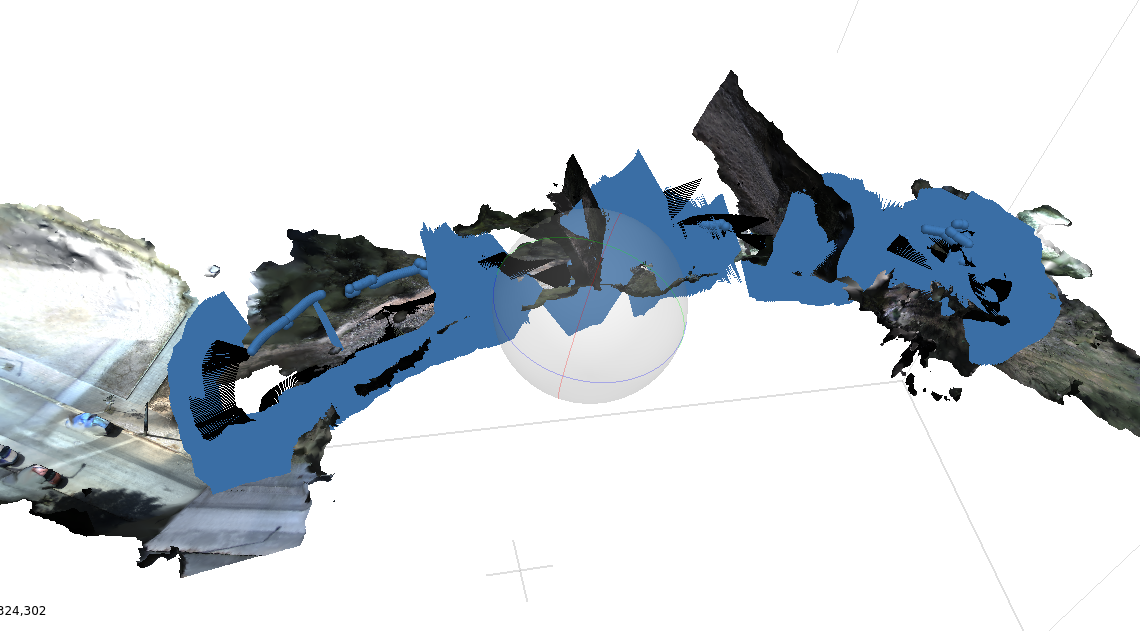
\includegraphics[width=0.45\textwidth]{figs/results/geometric_understanding/coimbra_zoomed_out.png}}
    \hfill
    \subfloat{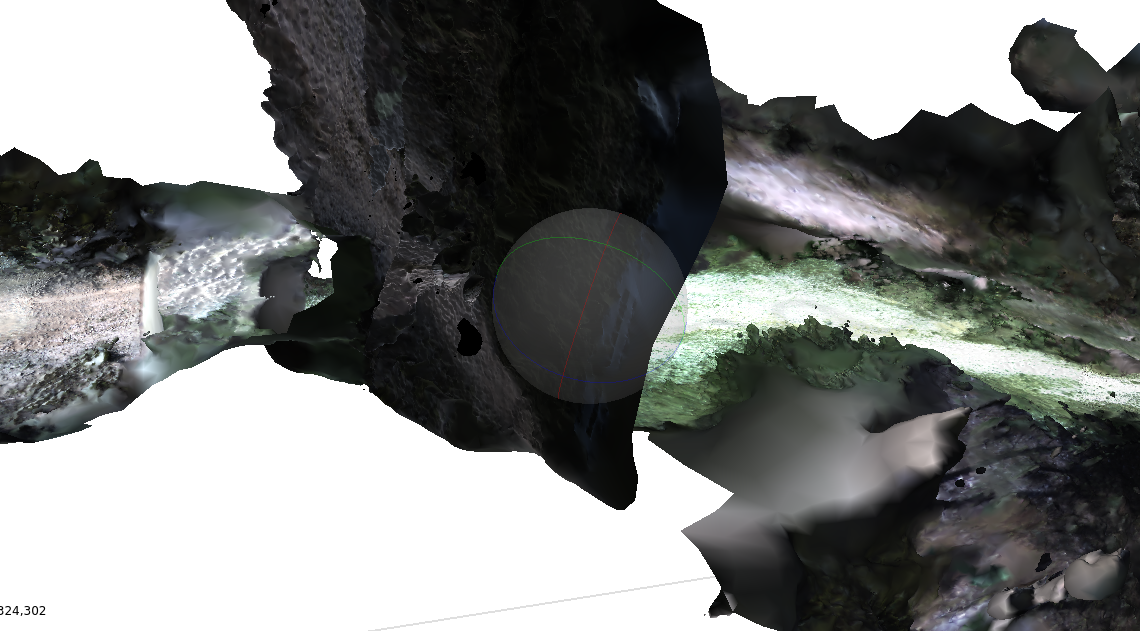
\includegraphics[width=0.45\textwidth]{figs/results/geometric_understanding/coimbra_zoomed_in.png}}
    \caption{3D reconstructions using Agisoft Metashape on three different environments. From top to bottom, they are a lawnmower pattern with a commodity drone,  The full map is shown to the left and a zoomed-in inset is shown to the right.}
    \label{fig:results:sfm}
\end{figure}

%A practical consideration when working with these systems is the camera exposure. This is generally handled well by commodity systems, but may need to be hand-tuned on an experimental robotic system. If the exposure is too long, especially in the case of rapid drone movement, there can be motion blur which degrades the quality of reconstructions. Similarlly, both over and under-exposed images lead to fewer features to match between images and areas of minimial information in the final mesh.  

\subsection{SLAM in Forest Environments}
We were interested in comparing the results of SLAM to photogrametry because these two systems represent an interesting tradeoff. SLAM approaches generally require multiple sychnronized and calibrated sensors, with LiDAR being a common requirement. However, they can run in an online manner which can be used to inform robots next actions. Photogrametery requires only images, with optional GPS. The downside is it is computationally expensive and must be run in a batch after all the images have been collected.

We conduct this comparison on the \textit{Gascola} dataset that was surveyed with lawnmower coverage and the custom payload at an off-nadir angle. We ran photogrametry using the default parameters. Francisco Yandun ran a tuned version of LIO-SAM and conducted the comparison between the two approaches.

As shown in Figure \ref{fig:results:slam_photogrametry_comparison}, the two maps agree fairly well in most regions. A notable source of high error is the tops of trees. In general, our qualitative assessment suggested that the SLAM approach was better at capturing these fine details compared to photogrametry. This is because it had the benefit of explicit 3D data from the LiDAR, while the photogrametery approach had to infer 3D information from images. This often leads to sharp points and fine detail being lost.


\begin{figure*}[h!]
   \centering
   %----primera subfigura----
   \subfloat[]{
        \label{fig:metashape_cloud_baseline}         %% Etiqueta para la primera subfigura
        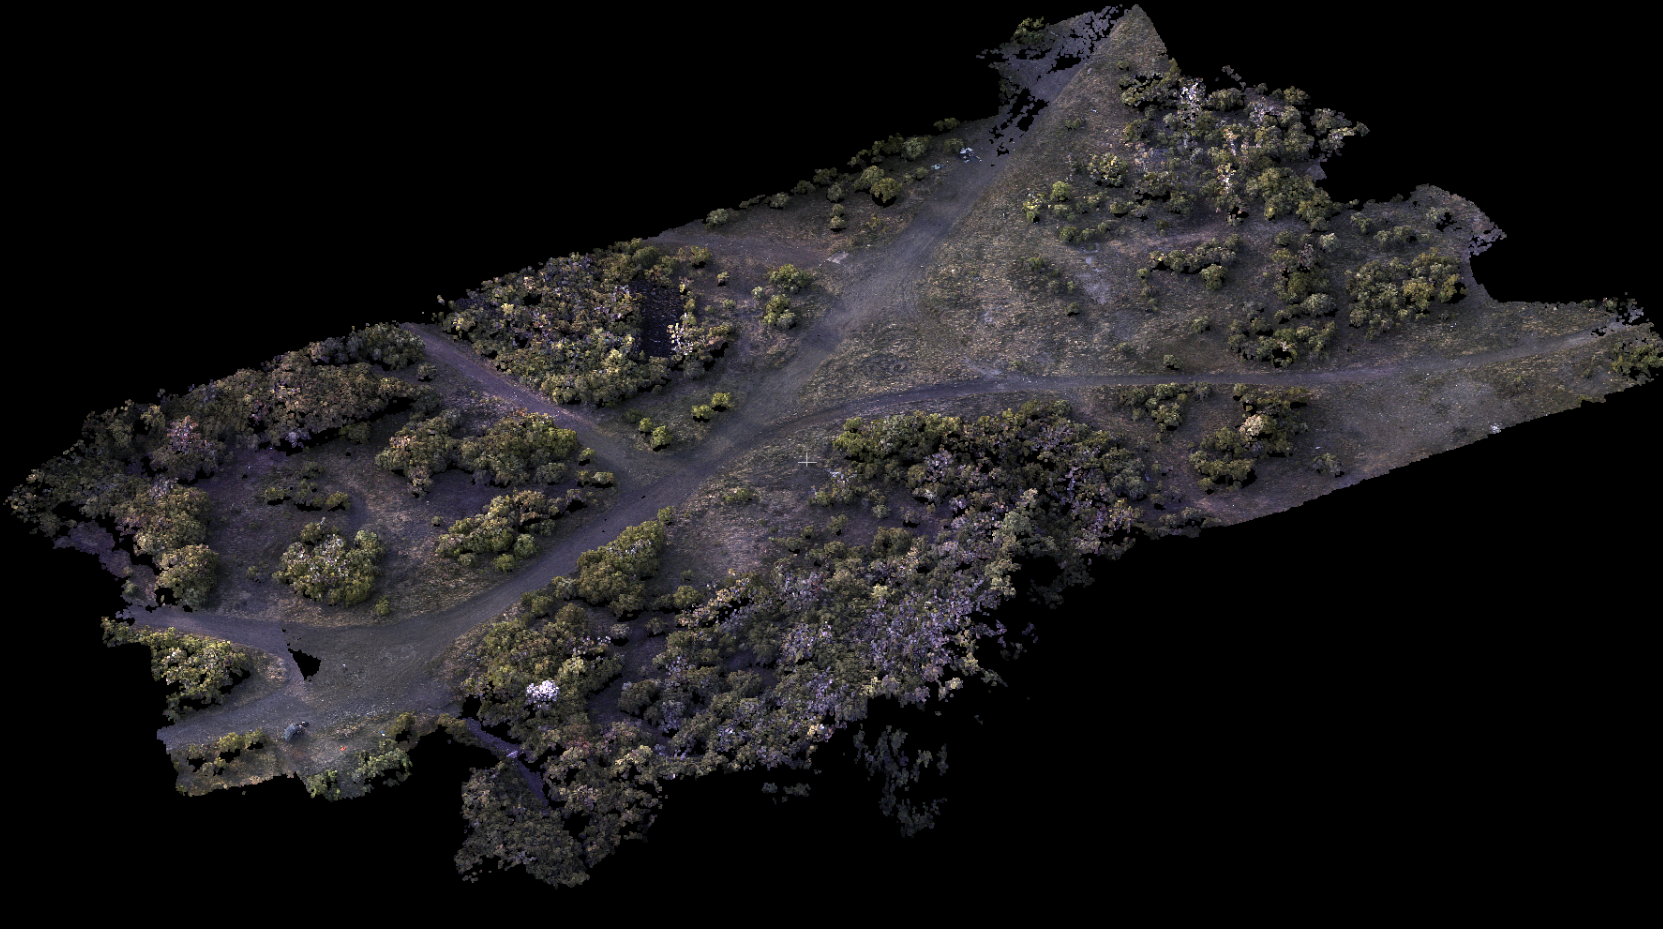
\includegraphics[width=0.465\textwidth]{figs/results/geometric_understanding/metashape_cloud_v3.png}}
   %\hspace{0.1\linewidth}
   \subfloat[]{
        \label{fig:slam_orig_1}         %% Etiqueta para la segunda subfigura
        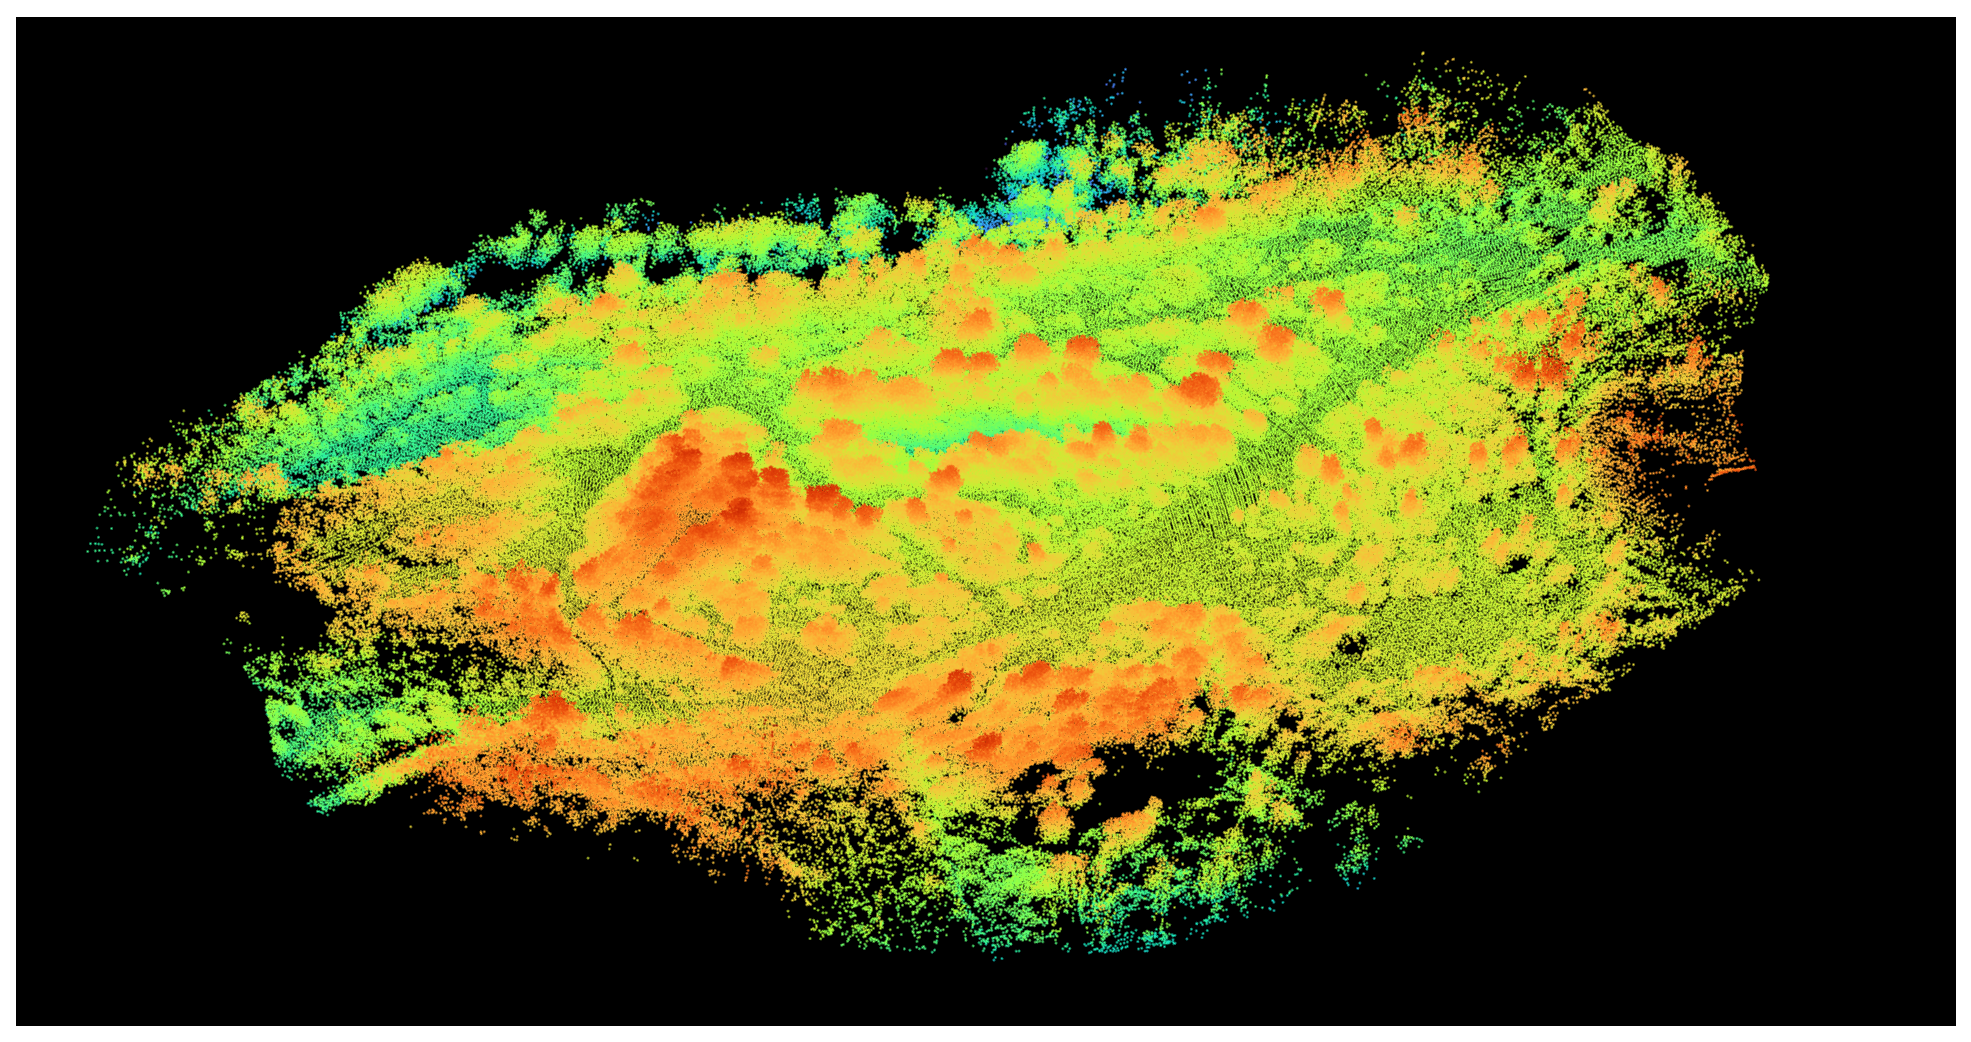
\includegraphics[width=0.5\textwidth]{figs/results/geometric_understanding/slam_ptCloud.eps}}\\%\\[20pt]   
   \subfloat[]{
        \label{fig:slam_hausdorff}         %% Etiqueta para la segunda subfigura
        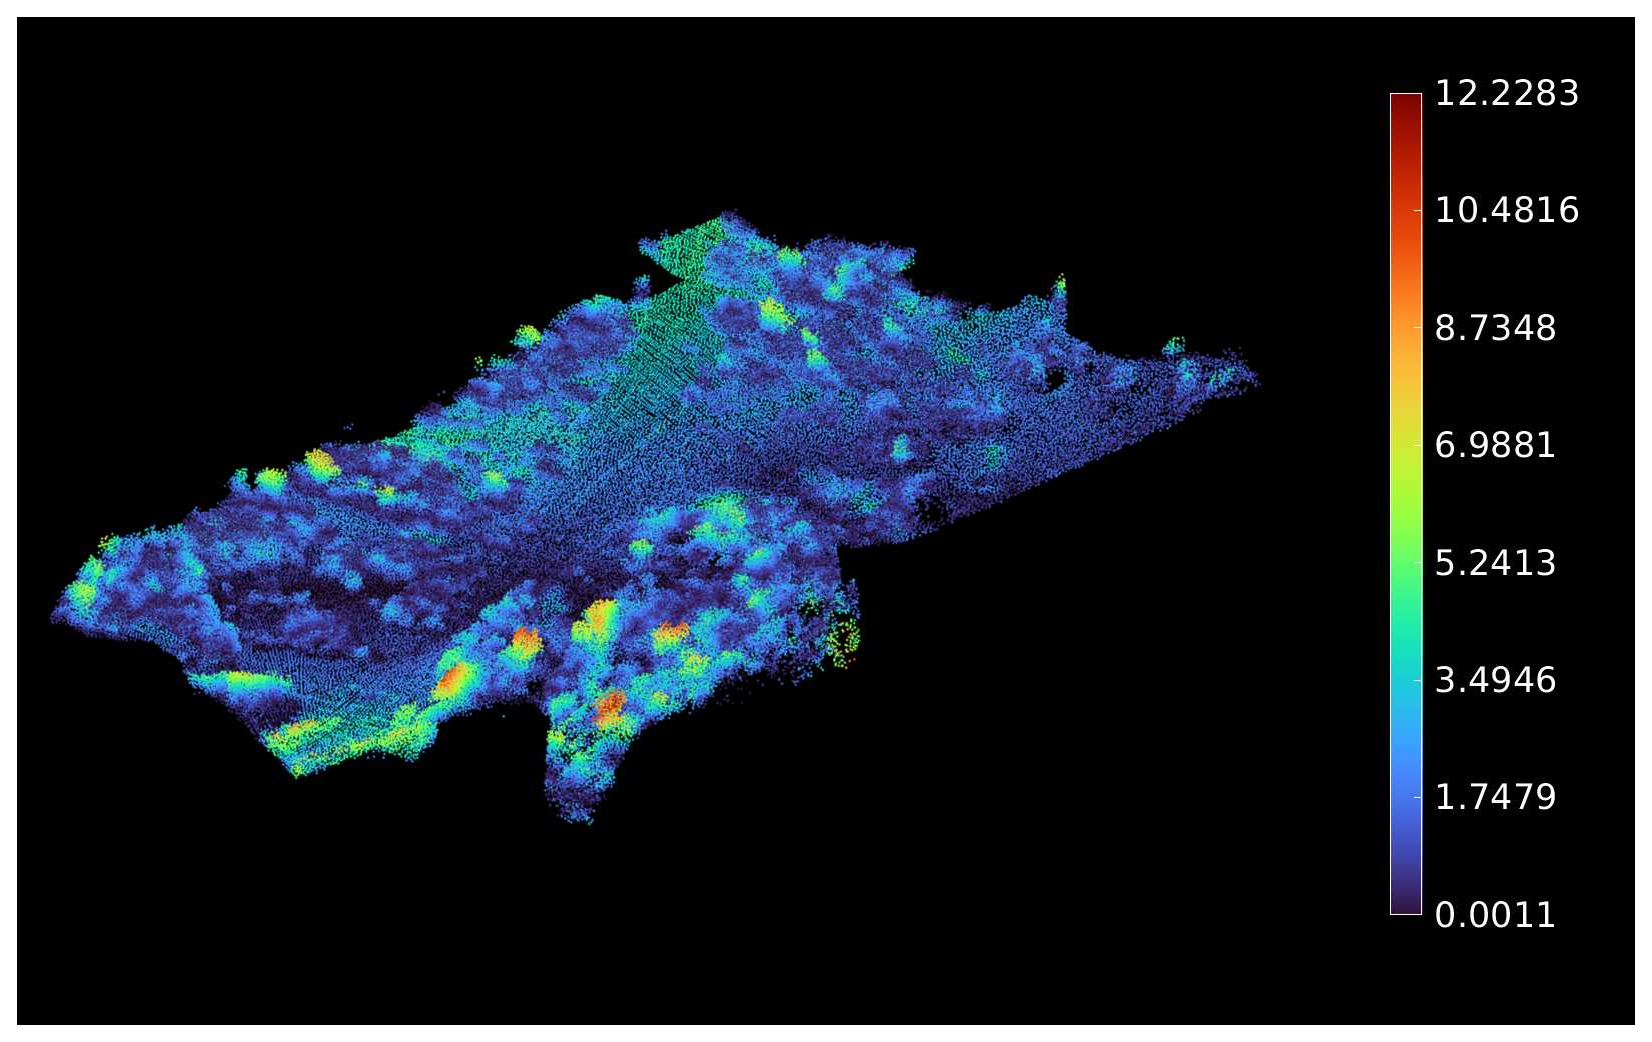
\includegraphics[width=0.5\textwidth]{figs/results/geometric_understanding/housedorff_distance.eps}}%\\[20pt]            
   \caption{Point cloud maps of the A) photogrammetry baseline, B) SLAM outcome. The two maps were compared using the Hausdorff distance, whose result is visualized as C) the SLAM map colored according to this metric. Note that the baseline and the SLAM clouds colormaps correspond to RGB and height values, respectively. Analysis and figure provided by Francisco Yandun.}
   \label{fig:results:slam_photogrametry_comparison}                %% Etiqueta para la figura entera
\end{figure*}

\section{Tree Detection using Data at Multiple Scales}
In this experiment we generate predictions on two different modalities from the same \textit{Stowe} cite. The first is an orthomosaic derived from the drone and the second is NAIP imagery derived from aerial data. These predictions are shown in Figure \ref{fig:results:tree_det}. 
The predictions on drone data appear significantly better than those from the NAIP data. This is unsurprising because of the increased detail provided by the higher resolution data. What is somewhat surprising is that fine-tuning the model did not appear to improve performance significantly. This motivates further analysis and quantitative evaluation of these results.

\begin{figure}[h]
    \subfloat{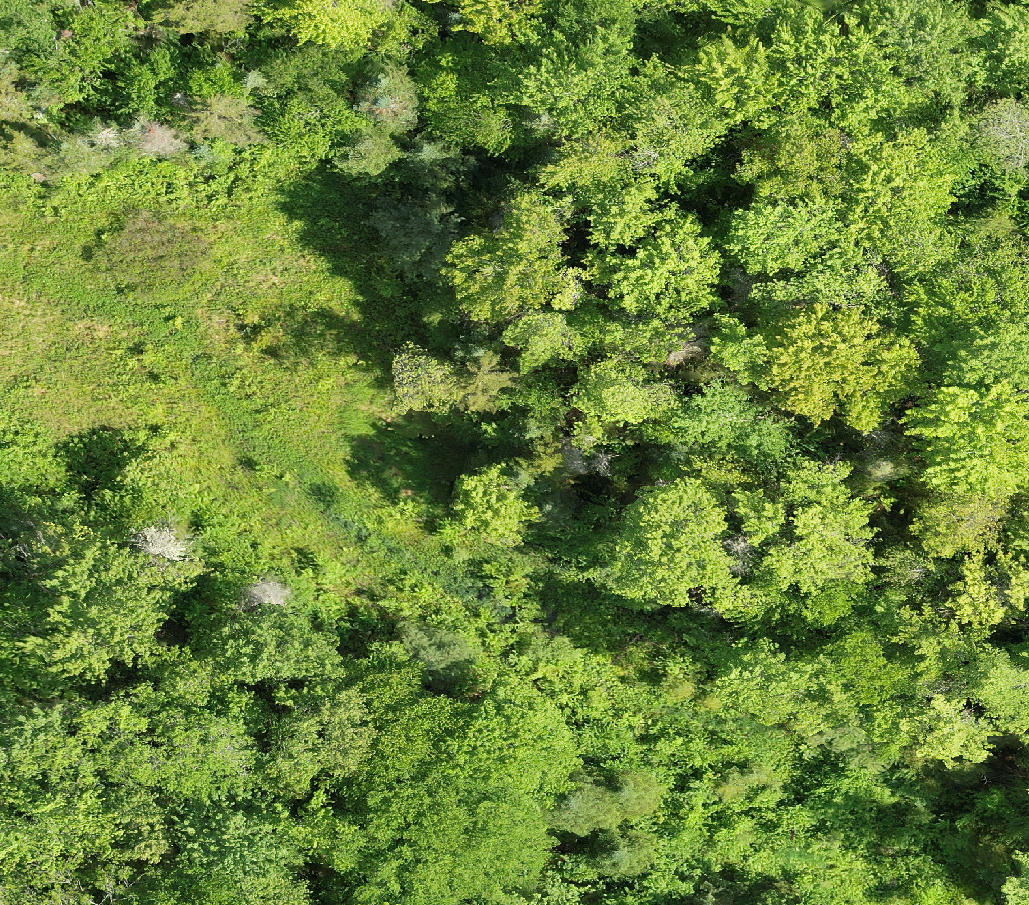
\includegraphics[width=0.40\textwidth]{figs/results/tree_detections/QGIS_VIS/base_image.png}}
    \hfill
    \subfloat{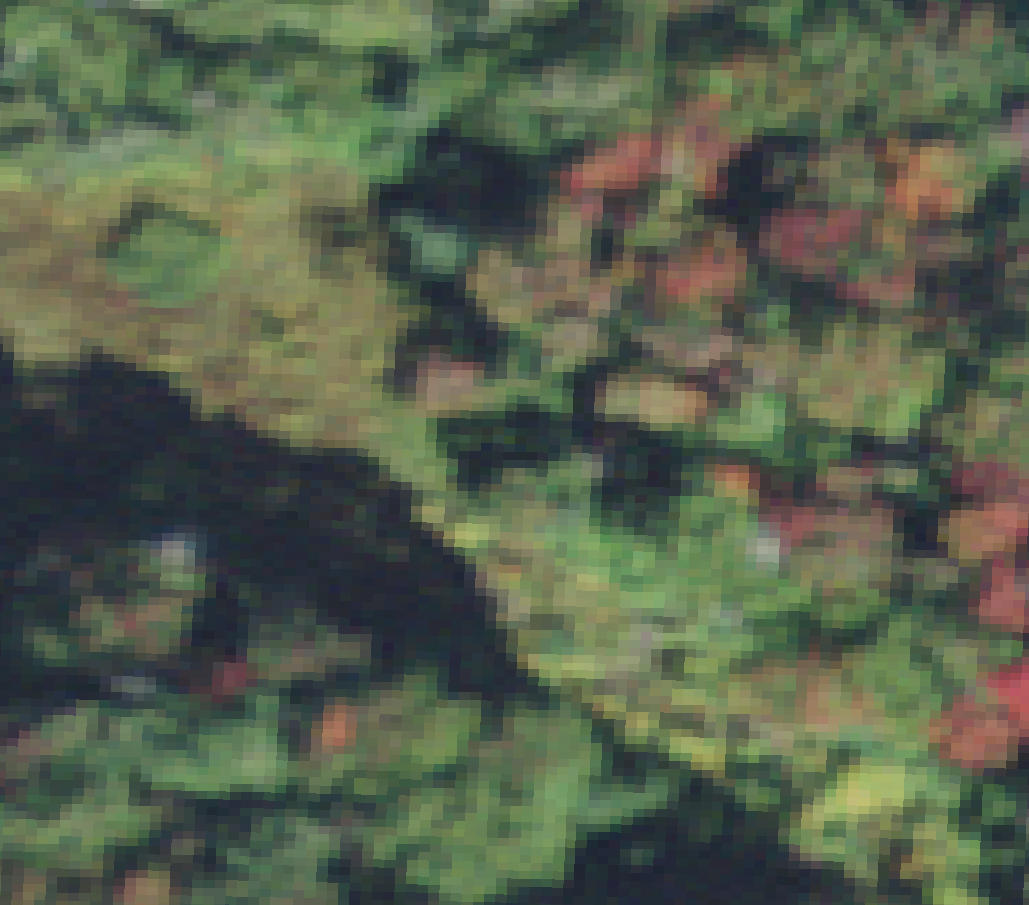
\includegraphics[width=0.40\textwidth]{figs/results/tree_detections/QGIS_VIS/naip_image.png}}
    \vfill
    \subfloat{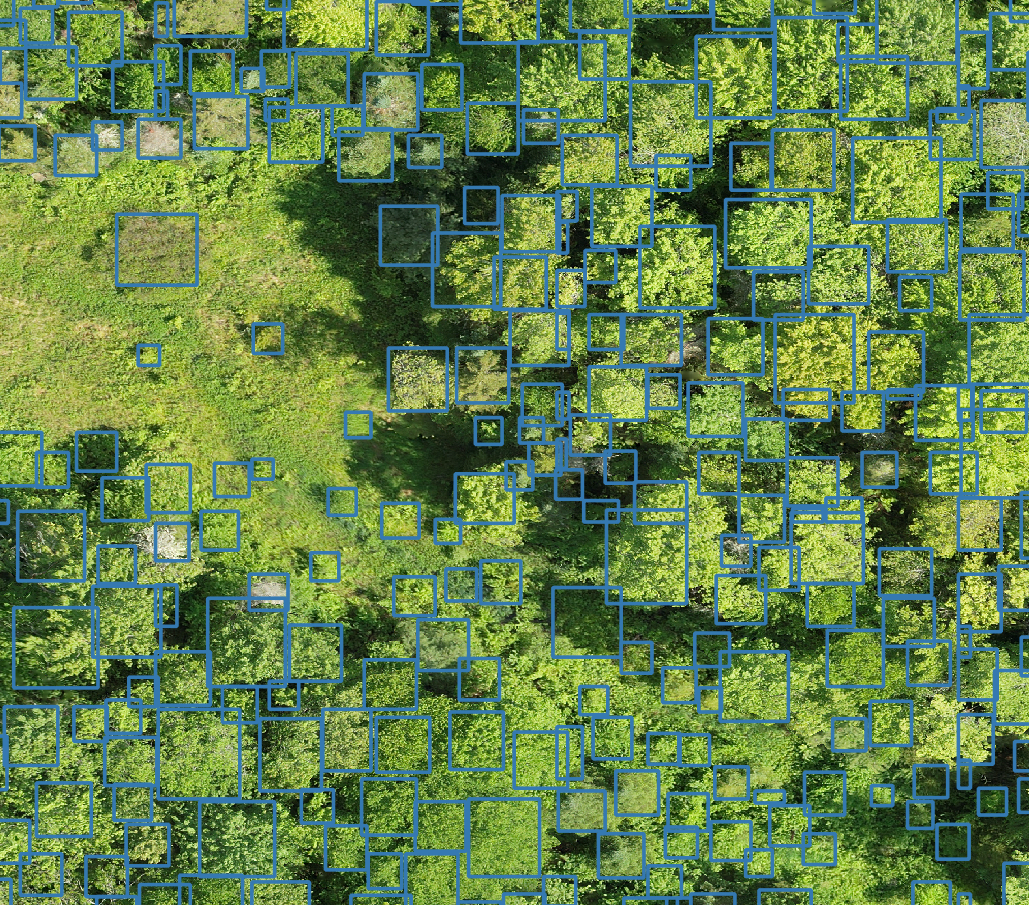
\includegraphics[width=0.40\textwidth]{figs/results/tree_detections/QGIS_VIS/drone_base.png}}
    \hfill
    \subfloat{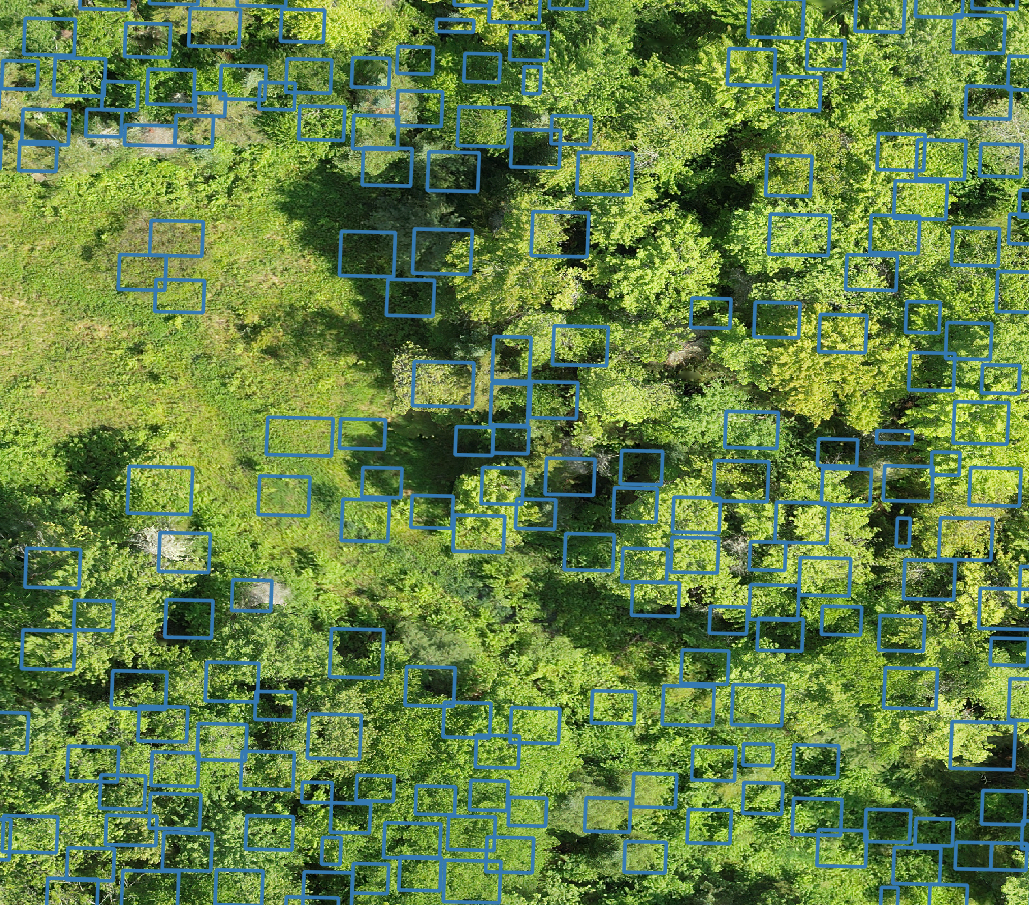
\includegraphics[width=0.40\textwidth]{figs/results/tree_detections/QGIS_VIS/naip_base.png}}
    \vfill
    \subfloat{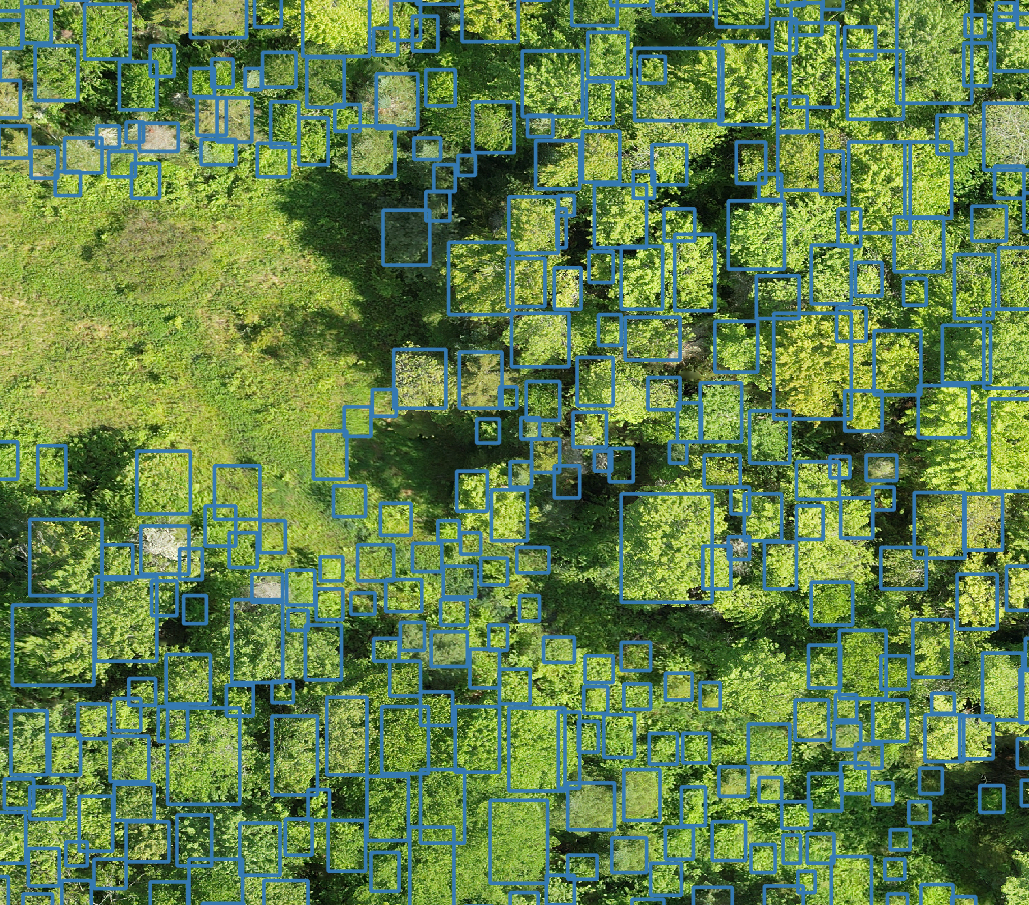
\includegraphics[width=0.40\textwidth]{figs/results/tree_detections/QGIS_VIS/drone_retrained.png}}
    \hfill
    \subfloat{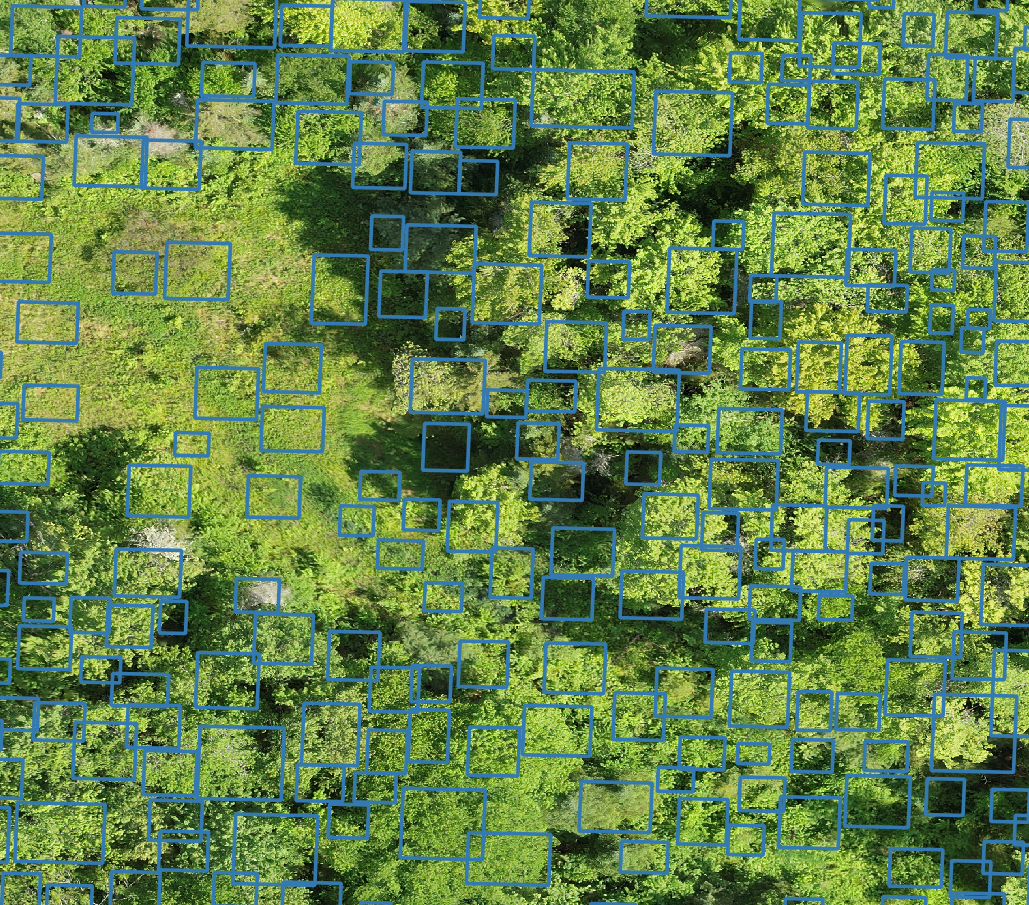
\includegraphics[width=0.40\textwidth]{figs/results/tree_detections/QGIS_VIS/naip_retrained.png}}
    \caption{Tree detections on a drone versus aerial data with and without fine-tuning on local data. Results for orthomosaics are on the left and NAIP is on the right. The first row is the input data, the second is the predictions from the base model, and the final is the predictions from the fine-tuned model. All predictions are visualized over drone data for clarity.
    }
    \label{fig:results:tree_det}
\end{figure}



\section{Semantic Mapping for Vegetation Classification}
The goal of this work is to build a 3D map of the environment that is annotated with the type of vegetation at each location. A challenge of this work is that we did not have access to field-reference data for the true locations of the different types of vegetatoin. Therefore, we conduct much of our quantitative evaluation on the semantic segmentation predictions, that can be more easily compared to human-labeled images. 

\subsection{Image Segmentation}
We conduct two experiments related to semantic segmentation. The first is a study using under-canopy data to determine the potential for synthetic pretraining and the impact of the number of training images on performance. The second is an evaluation of the model we used in over-canopy mapping with a small set of training examples.
\subsubsection{Sete Fonte Experiment}

\begin{figure}
    \centering
    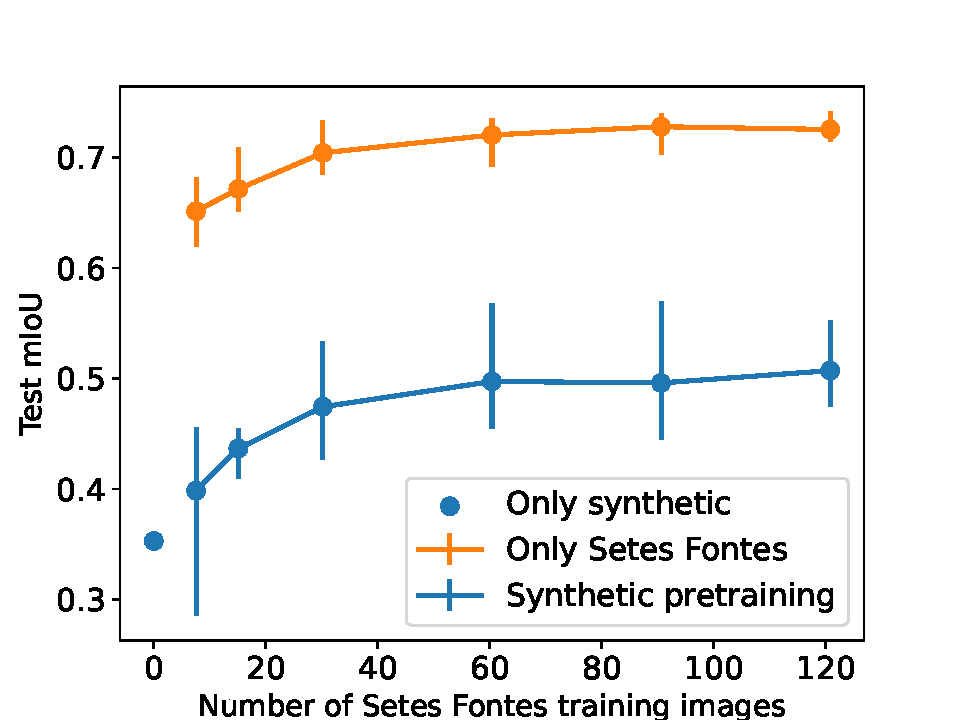
\includegraphics[width=0.7\textwidth]{figs/results/semantic_segmentation/synthetic_experiments_mious.pdf}
    \caption{Test mIoU for very few training images on the \textit{Setes Fontes} dataset.
    Error bars represent minimum and maximum result across the five folds of \textit{Setes Fontes}.}
    \label{fig:results:semantic-size-pretraining}
\end{figure}

In this experiment, we compare a model trained just on synthetic data from \textit{Synthetic}, models pretrained on \textit{Synthetic} and then increasing ammounts of real data, and models trained solely on increasing ammounts of real data. The mean Intersection over Union on the test set of each of these configurations is shown in Figure \ref{fig:results:semantic-size-pretraining}.
It is interesting to note the relatively high performance of a model that used only 7 real images. Also, the model trained solely on synthetic data fails to generalize to real data, even after properly accounting for differences in mean and variance of both datasets. We found that combined real and synthetic data performs worse than training the same model only using real data. This suggests that the synthetic data comes from a completely different distribution than the real one, making its contribution detrimental. In the future, we plan to keep researching the causes of this interesting outcome.
\begin{figure}
    \centering
    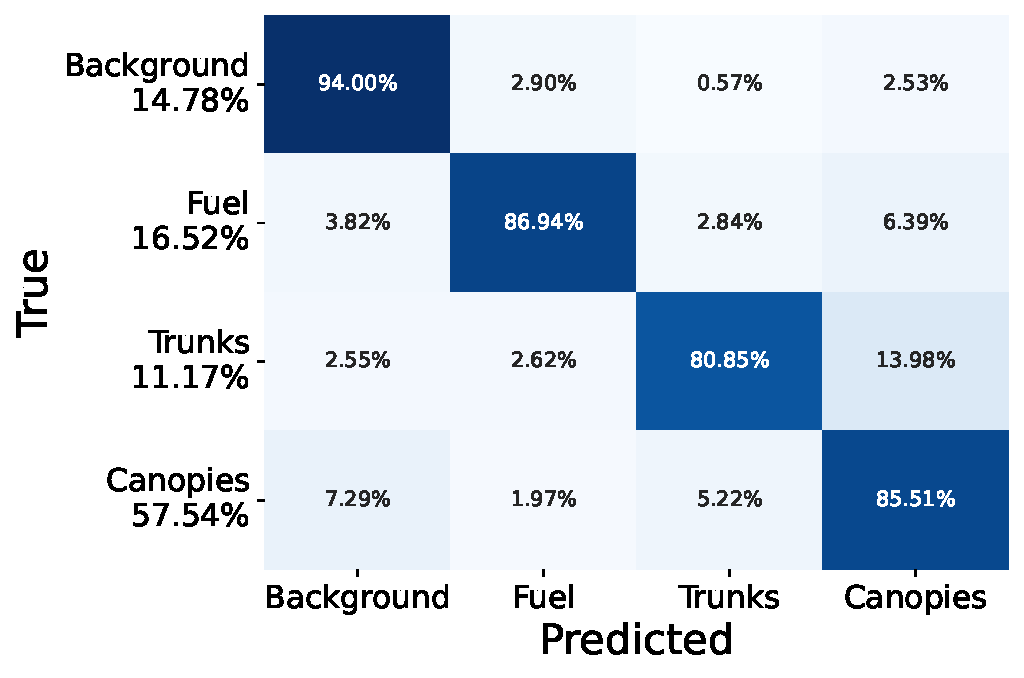
\includegraphics[width=0.7\columnwidth]{figs/results/semantic_segmentation/confusion_matrix.pdf} 
    \caption{Confusion matrix for the \textit{Setes Fontes} test datasets normalized per class with the true fraction of each class reported on the y axis labels.
    %Fuel is predicted fairly well, though it is fairly often confused for canopy, which is understandable given the visual similarity and the large fraction of canopy pixels.
    }
    \label{fig:results:sete_fontes_confusion_matrix}
\end{figure}

Since the model trained in 121 images ($80\%$ of the \textit{Setes Fontes} dataset) showed the best performance in these experiments, we conducted further experiments on it. The confusion matrix on the \textit{Sete Fontes} test set is shown in Figure \ref{fig:results:sete_fontes_confusion_matrix}. This shows that all four classes are predicted with reasonable accuracy. A common source of confusion is between trunks and canopies, which is understandable because they frequently overlap. Canopies are also confused for background, which includes sky. Even though these two classes look very different, sky can often be seen through the canopy, and the network miss-classifies these fine details. In most cases, this error is harmless because no LiDAR information should correspond to the sky pixels. Finally, the most common error for fuel is canopies, which is understandable because they are both leafy vegetation. Information about the height, either provided to the model or used in post-processing, could help disambiguate this confusion. 

Since we are mainly interested in the fuel instances, we aggregated the background, trunks, and canopies in a single non-fuel class. In that case we obtained an IoU of 78.2\% and 95.3\% for \texttt{Fuel} and \texttt{Not Fuel}, respectively, which yields a mIoU of 86.7\%. This shows that our system performs well at its primary task of identifying fuel.

\begin{figure}
   % First row
   \centering
    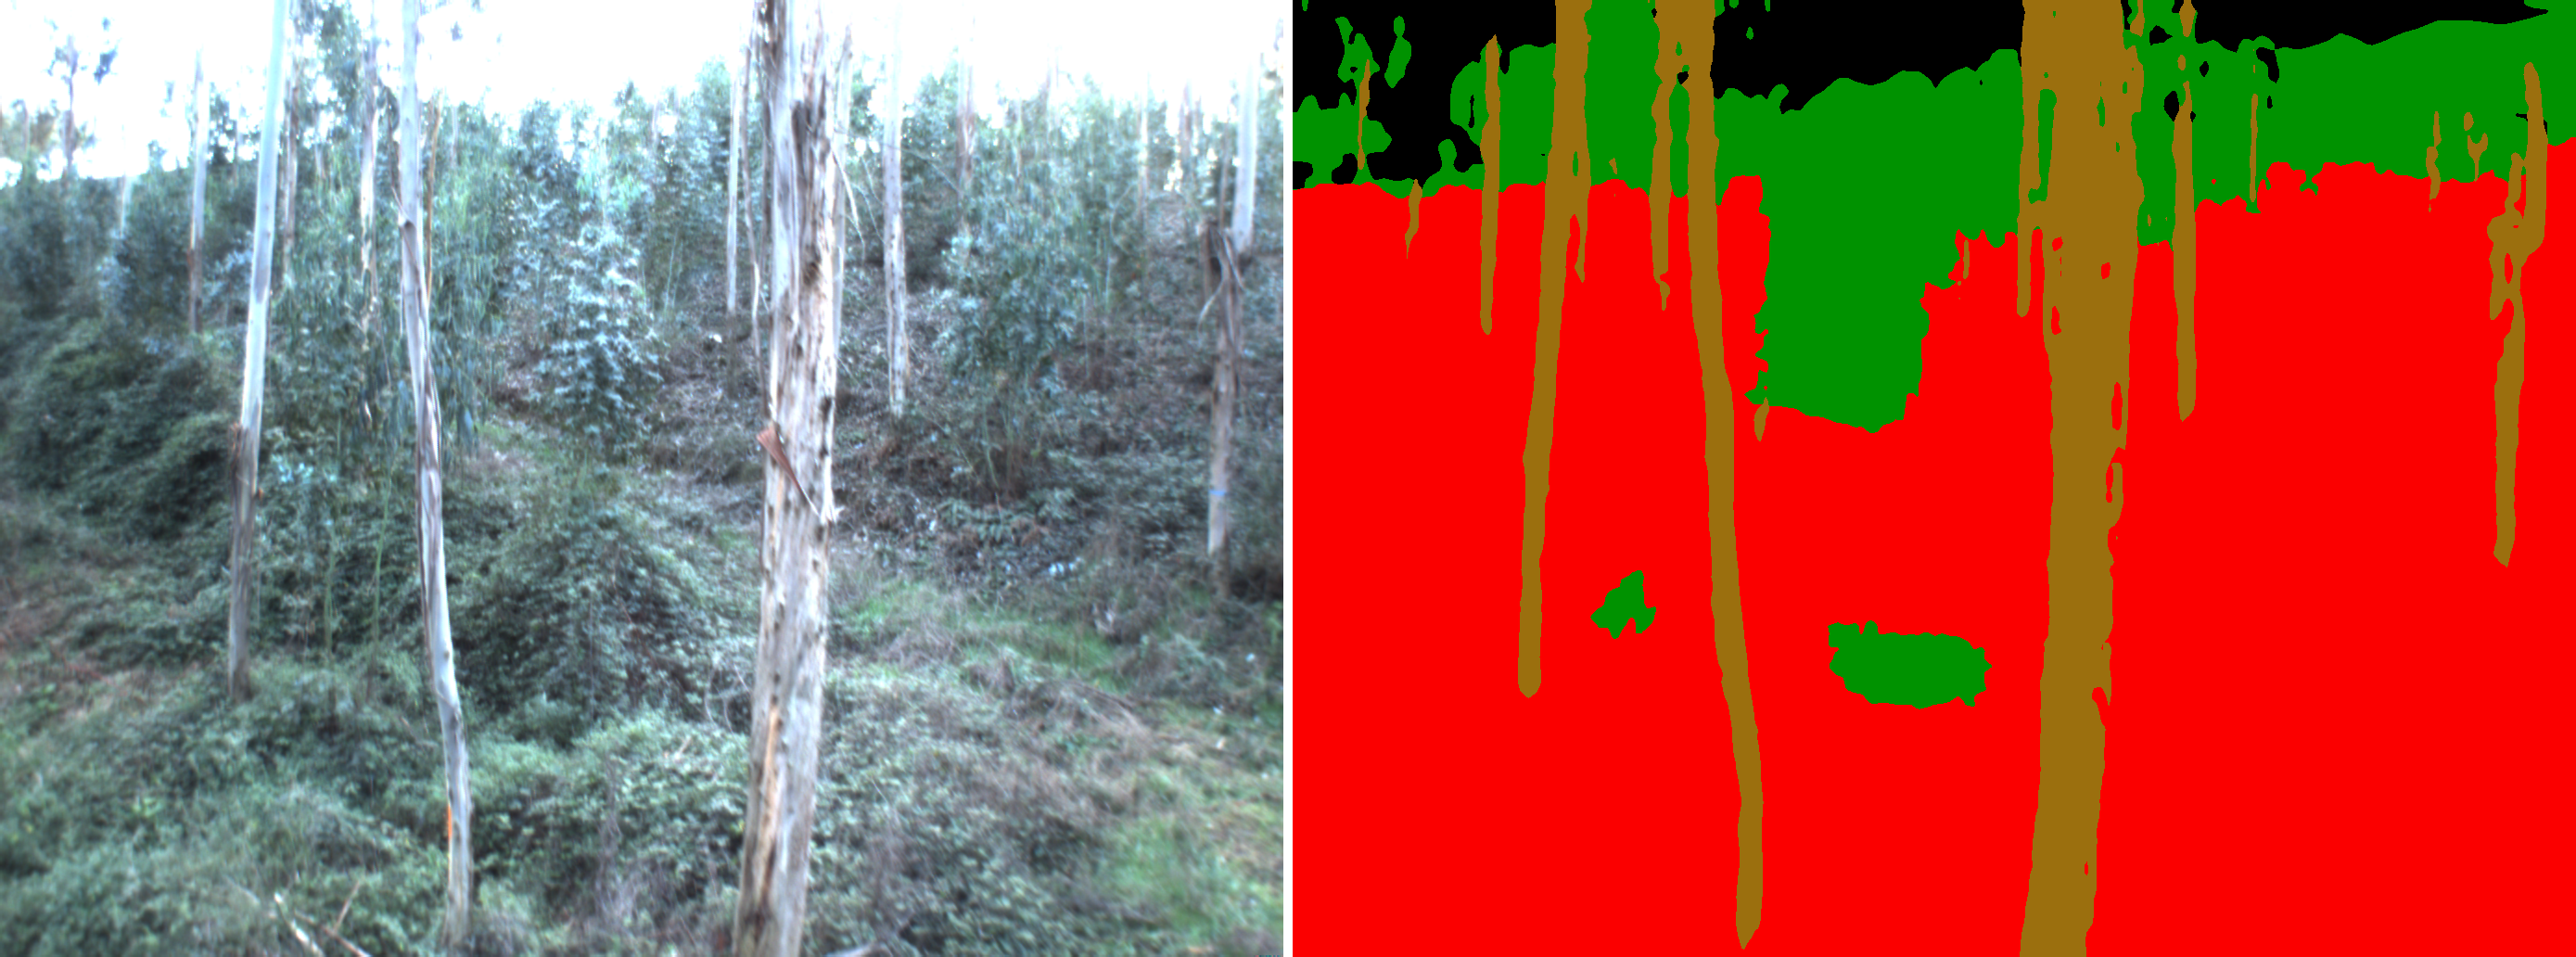
\includegraphics[width=\linewidth]{figs/results/semantic_segmentation/SeteFontes/qualatative_001400.png}  
    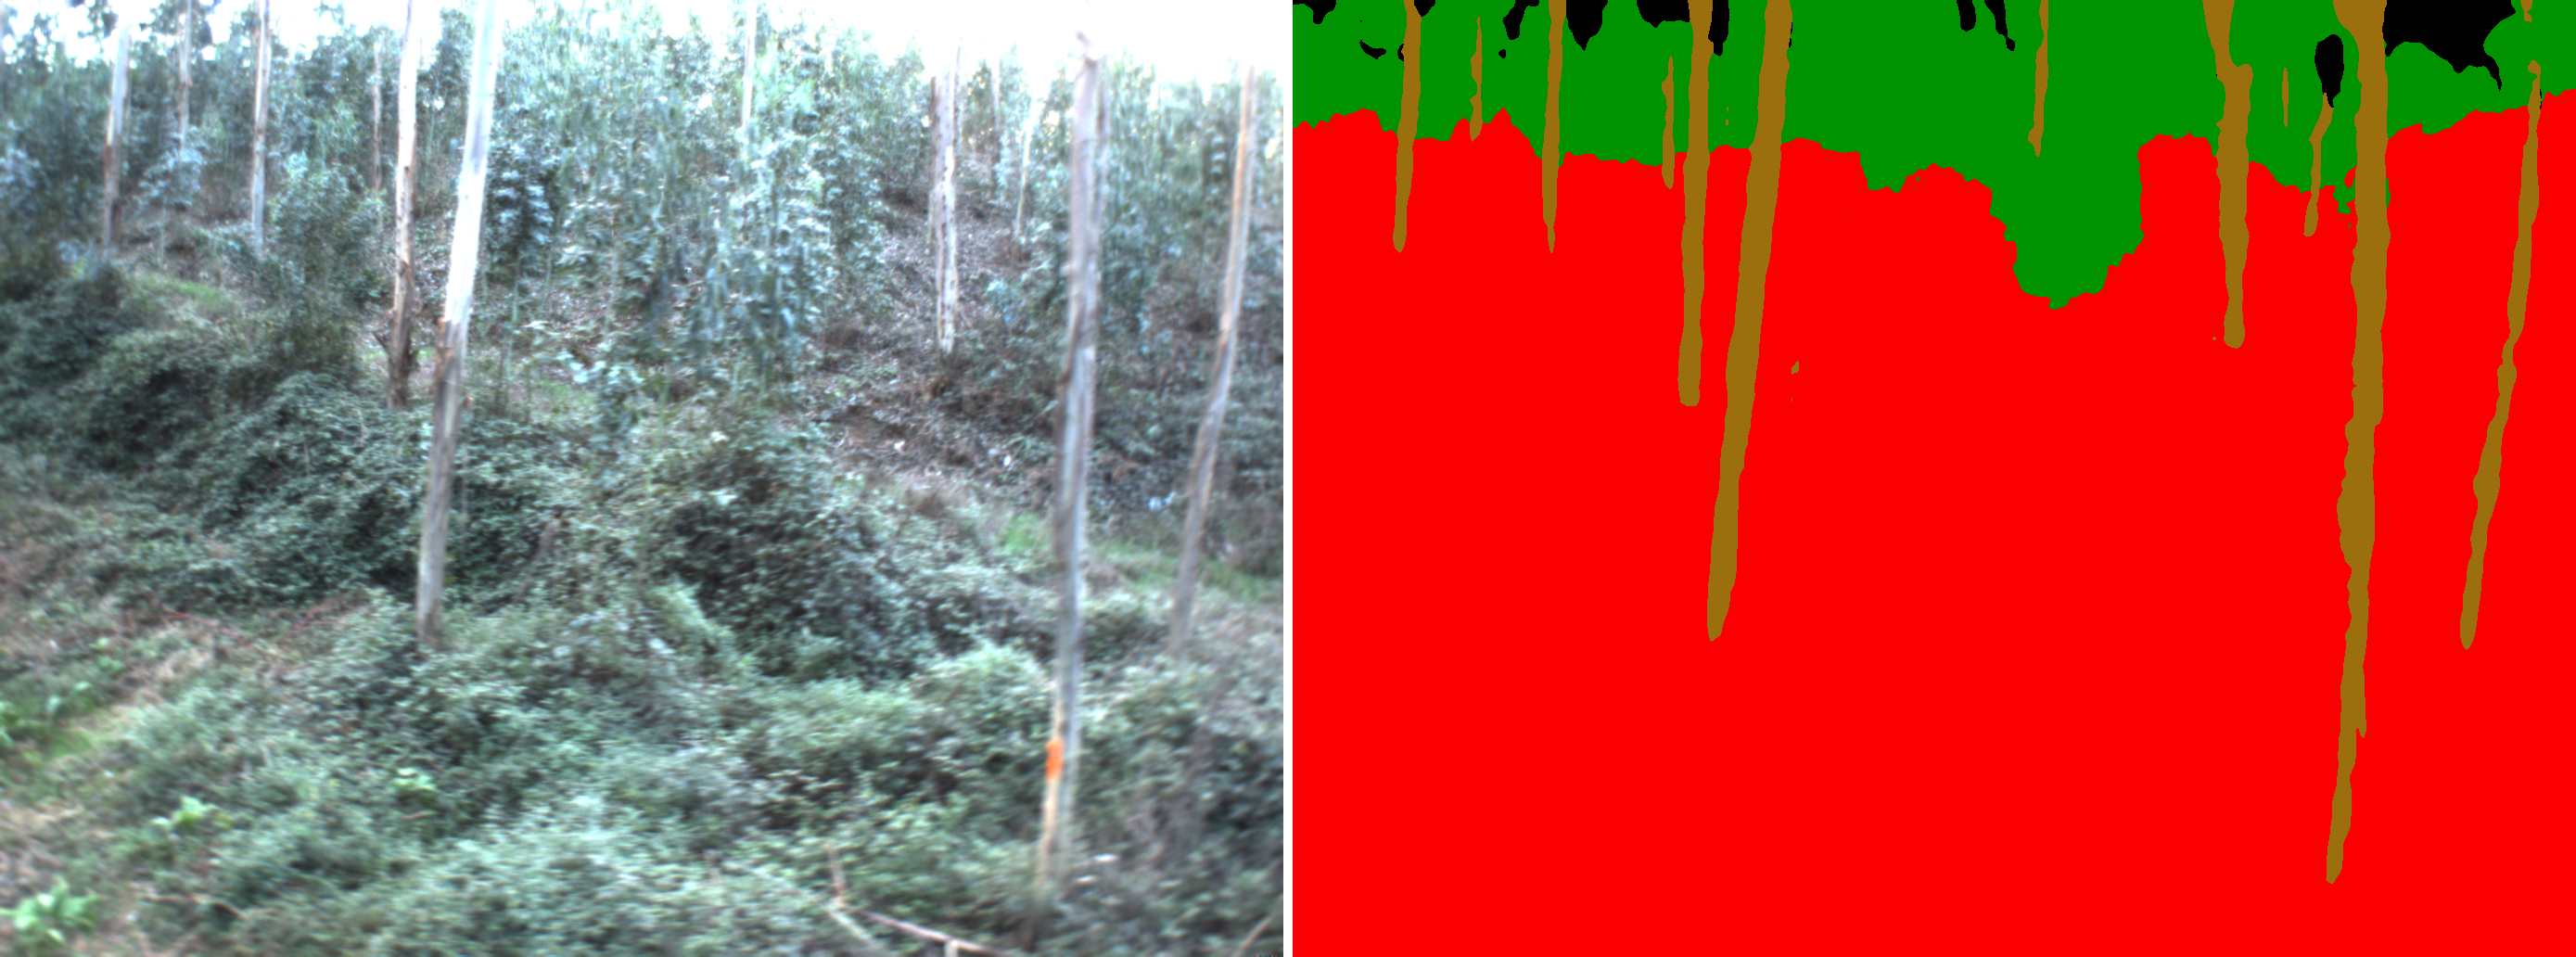
\includegraphics[width=\linewidth]{figs/results/semantic_segmentation/SeteFontes/qualatative_001600.png}  
    \caption{Predictions on the \textit{Oporto} dataset. Black is background, red is fuel, brown is trunks, and green is canopy.
    %Note that low trees are often predicted as fuel.
    } 
    \label{fig:results:oporto_semantic_seg_qual}
\end{figure}


The end goal of this model is to be useful on the semantic mapping task on the \textit{Oporto} dataset, that wasn't seen during training. We show two qualitative examples of predictions in Figure \ref{fig:results:oporto_semantic_seg_qual}. The predictions still appear fairly accurate, despite the change in camera perspective from ground to aerial and different images characteristics. 


\subsubsection{Gascola Experiment}
In this experiment, we used two different datasets from \textit{Gascola} which partially covered the same region. We train on one dataset and test the model on the other. Because of the small number of images that we used in this experiment, these two datasets had different class distributions as shown in Figure \ref{fig:results:semantic_class_fracs}, though they had the same three main classes. Each of these three classes corresponded to a different aggregate class (Background, Canopy, and Fuel), so it was important to effectively tell them apart. 


\begin{figure*}[h!]
   \centering
   %----primera subfigura----
   \subfloat[]{
        \label{fig:train_class_frac}         %% Etiqueta para la primera subfigura
        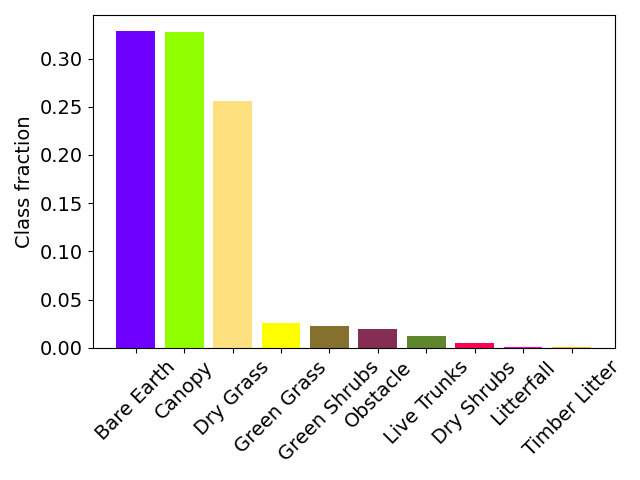
\includegraphics[width=0.5\textwidth]{figs/results/semantic_segmentation/class_fraction_train.png}}
   %\hspace{0.1\linewidth}
   \subfloat[]{
        \label{fig:test_class_frac}         %% Etiqueta para la segunda subfigura
        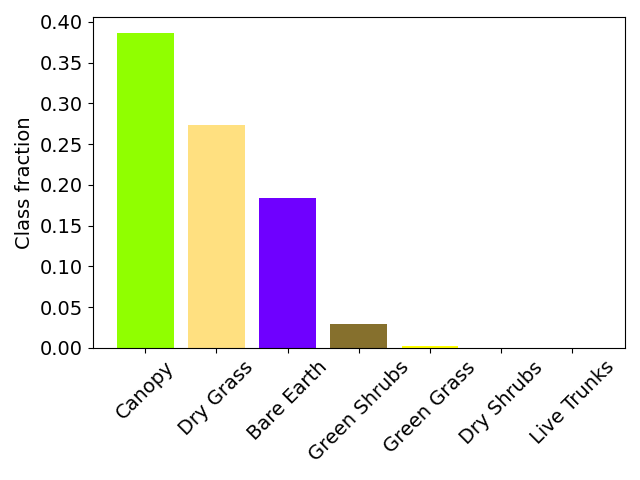
\includegraphics[width=0.5\textwidth]{figs/results/semantic_segmentation/class_fraction_test.png}}%\\[20pt]            
   \caption{This shows the fraction of pixels per class for A) the train set and B) the test set. Note that the three dominant classes Canopy, Bare Earth, and Dry Grass are common across both collections but the comparative frequencies are somewhat different. These correspond to our aggregate Canopy, Background, and Fuel classes respectively. The fractions of other classes are fairly small, and some from the training set are entirely absent in the test set.}
   \label{fig:results:semantic_class_fracs}                %% Etiqueta para la figura entera
\end{figure*}

The quality of predictions is shown in Table \ref{tab:results:semantic_eval}. The the performance is fairly good on the most common classes, but, as expected drops on the rarer classes. As seen by the qualitative examples in Figure \ref{fig:results:semantic_gascola_qualitative}, there are instances where the predictions on the granular classes are incorrect, but the aggregate class is correct.

\begin{table}[ht!]
    \centering
\begin{tabular}{ccccc}
% \hline
\toprule
\textbf{Class} & \textbf{IoU} & \textbf{Precision} & \textbf{Recall} \\ \midrule
% \hline
Canopy & 70.05 & 84.77 & 80.13 \\
Dry Grass & 79.7 & 93.75 & 84.17 \\
Bare Earth & 78.53 & 88.12 & 87.83 \\
Green Shrubs & 3.27 & 21.72 & 3.71 \\
Green Grass & 0.0 & 0.0 & 0.0 \\
Dry Shrubs & 0.0 & 0.0 & 0.0 \\
Live Trunks & 0.05 & 0.05 & 84.09 \\
\bottomrule
% \hline
\end{tabular}
\caption{Evaluation results of the SegNext \cite{} network with the Anderson Fuel Model as a base for semantic segmentation in a forestry environment.}
\label{tab:results:semantic_eval}
\end{table}


\begin{figure*}[h!]
   \centering
   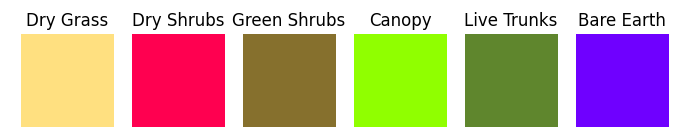
\includegraphics[width=0.5\textwidth]{figs/results/semantic_segmentation/Gascola/safeforest_all_classes_flat.png}
   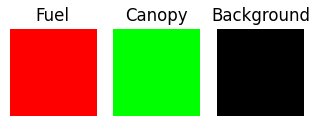
\includegraphics[width=0.25\textwidth]{figs/results/semantic_segmentation/Gascola/safeforest_classmap_compressed_flat.png}
   \includegraphics[width=0.80\textwidth]{figs/results/semantic_segmentation/Gascola/000000_rgb_img.png}
   \vspace{0pt}
   \includegraphics[width=0.80\textwidth]{figs/results/semantic_segmentation/Gascola/000005_rgb_img.png}
   \vspace{0pt}
   \includegraphics[width=0.80\textwidth]{figs/results/semantic_segmentation/Gascola/000010_rgb_img.png}
   \vspace{0pt}
   \includegraphics[width=0.80\textwidth]{figs/results/semantic_segmentation/Gascola/000015_rgb_img.png}
   \vspace{0pt}
   \caption{
   Qualitative semantic mapping results from the test set. The results are shown both for the predicted classes and the aggregated ones, with colors visualized in the top rows.
   White regions in the ground truth represent areas that were ambiguous to the human annotator. Overall the predictions match the ground truth well and boundaries are well-defined. Note that many regions of confusions, such as canopy-to-trunk and green shrub to canopy, fall within the same coarse classes for our mapping purposes.
   }
   \label{fig:results:semantic_gascola_qualitative}                %% Etiqueta para la figura entera
\end{figure*}

\subsection{Projecting Segmentation into 3D}
The final goal of semantic mapping is to develop a model of the environment and what class different regions are. To evaluate the feasibility of this, we conduct two experiments using multi-sensor data.

The first experiment is conducted on the \textit{Oporto} dataset, which is collected in a clearing in Portugal with the custom payload at an orientation of 30 degrees from horizontal. For semantic segmentation we use the model trained on \textit{Sete Fontes}. For localization, we use the vision-LiDAR SLAM system from \cite{RussellUnmannedMitigation}.
The results are shown in Figure \ref{fig:results:semantic_mapping_original}. This shows that the system was able to determine that there was significant fuel at ground level and correctly identify the tree trunks in the environment. The later is important because trunks could be used as a localization aid in a similar way to SLOAM \cite{Chen2020SLOAM:Inventory}. One issue that we observed was that multiple scans were not perfectly registered to each other. This is in contrast to the final pointcloud derived from SLAM, where fine details are captured precisely. Our hypothesis is that because the SLAM system uses a pose-graph \cite{Dellaert2017FactorPerception} formulation, information from loop closures can be used to update the historical pose to make it more accurate. However, the semantic mapping system only uses the most recent SLAM pose estimate, which is likely to be less accurate than the final optimized version.

\begin{figure}
    \centering
    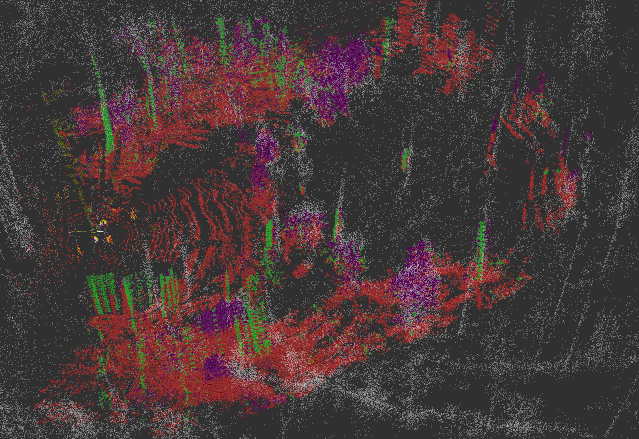
\includegraphics[width=0.8\textwidth]{figs/results/semantic_mapping/semantic_cloud_first_approach.png}
    \caption{Semantic mapping results on the Oporto test site. Fuel is red, trunks are green, canopy is purple, and background is black. White points are unlabeled.}
    \label{fig:results:semantic_mapping_original}
\end{figure}

A limitation of the first experiment was our lack of ground truth data to compare against.
In our second experiment on the \textit{Gascola} dataset, we still did not have field reference data, but tried to approximate this as accurately as possible.
We choose to label an ortho-mosoaic derived from a 3D model by hand. We used QGis \cite{QGIS_software}, an open-source software for interacting with geospatial data. We labeled three coarse classes, fuel, canopy and background, which included bare-earth and other non-flammable material. Trunks were not included because they could almost never be observed in the top-down view from the orthomosaic. This manual process took approximately eight hours to complete and is visualized on the left side of Figure \ref{fig:results:semantic_map_UFO}.

In this experiment, we used the SegNext model trained on the manually-labeled dataset from the flight we were not using for mapping. We used the localization LIO-SAM \cite{} and provided by Franciso Yandun to estimate pose. In this case, we used UFOMap instead of octomap to aggreate the observations, because of the improved performance. This change was implemented by Duda Andrada and she conducted the experiments reported here. There results of this are shown in Figure \ref{fig:results:semantic_map_UFO}. The overall structure of the scene matches well and small local features are correctly identified. One major source of error is seen in the miss-registration of data from adjacent drone flights. This is seen in the vertical offsets that are especially visible on the left side of the map. This may be due to latency in the processing or also because of using the un-refined pose as described previously. The quality of this result suggests that with additional work to properly register the scans, this system could be a powerful tool for vegetation mapping. 

\begin{figure}
    \centering
    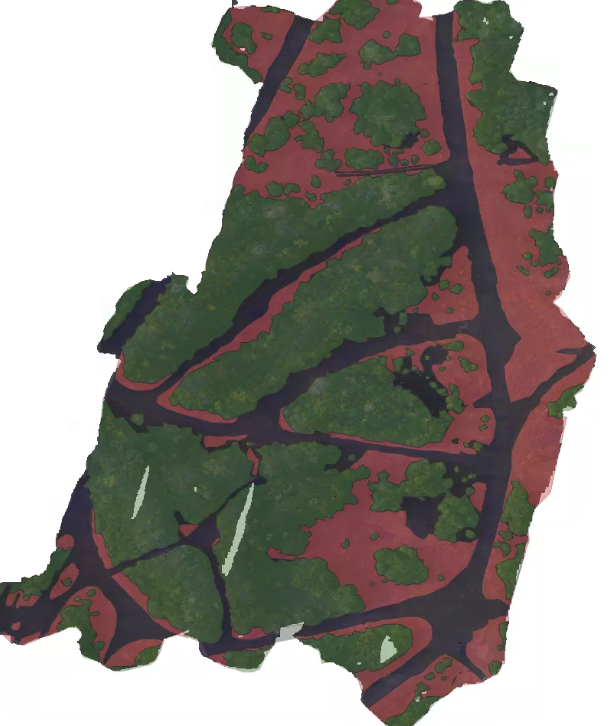
\includegraphics[width=0.45\textwidth]{figs/results/semantic_mapping/labeled_orthomoasaic.png}
    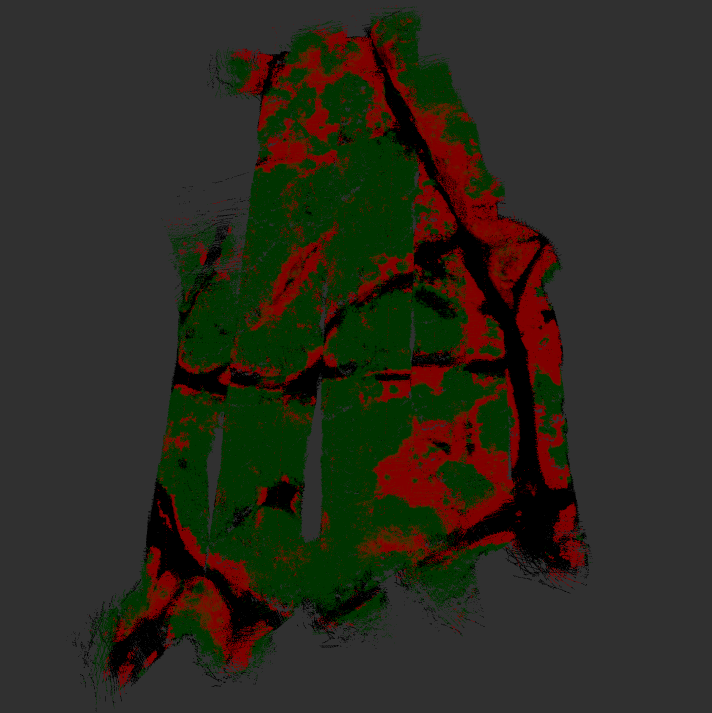
\includegraphics[width=0.45\textwidth]{figs/results/semantic_mapping/segnext_gc5_ufomap.png}
    \caption{Manually-labeled result on the left, result from UFO-Map on the right provided by M. Duda Andrada, using the SegNext model trained on Gascola Data.}
    \label{fig:results:semantic_map_UFO}
\end{figure}


\section{Informative Path Planning for Commodity Drones}
We evaluate the informative path planning approach on an area near Herndon, VA. This has a mix of farmfield and forest, with occasional buildings and roads. As seen in Figure~\ref{fig:results:ipp_paired}, when run on the same data, the proposed approach is able to come up with a plan that yields a more representative sample of the environment, compared to the baseline. Further examples of the proposed planning method run on image data can be seen in Figure~\ref{fig:results:ipp_unpairqual}. 

\begin{figure}[h]
    \subfloat{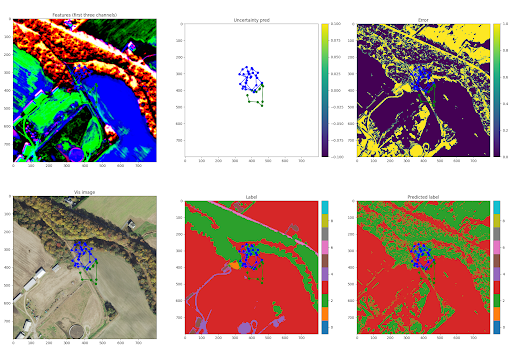
\includegraphics[width=0.45\textwidth]{figs/results/ipp/unpaired_qual_1 (1).png}}
    \hfill
    \subfloat{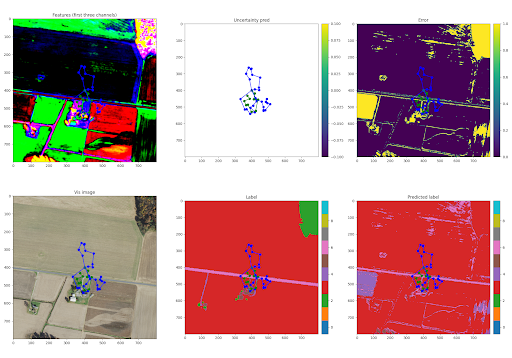
\includegraphics[width=0.45\textwidth]{figs/results/ipp/unpaired_qual_2 (1).png}}
    \caption{Visualizations of the proposed planning method on two different data images.}
    \label{fig:results:ipp_unpairqual}
\end{figure}


\begin{figure}[h]
    \subfloat{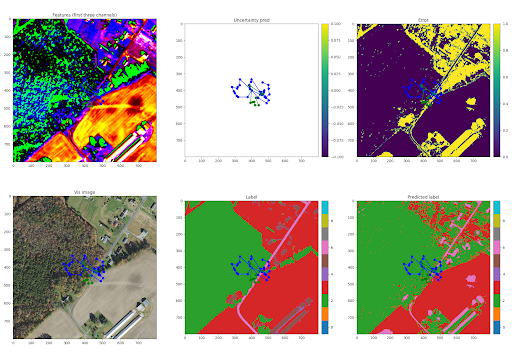
\includegraphics[width=0.45\textwidth]{figs/results/ipp/paired_qual_GBS-IPP (1).png}}
    \hfill
    \subfloat{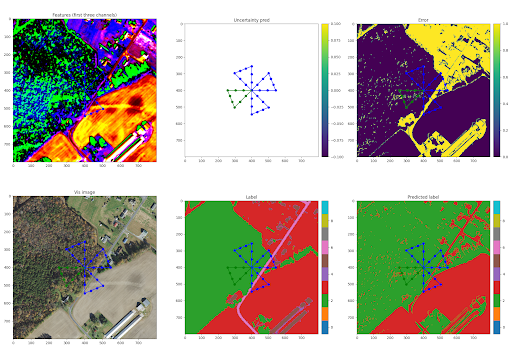
\includegraphics[width=0.45\textwidth]{figs/results/ipp/paired_qual_pizza (1).png}}
    \caption{A comparison of the proposed method with a baseline}
    \label{fig:results:ipp_paired}
\end{figure}

The experiments demonstrate a small but significant improvement in both error metrics from the proposed, as can be seen in Figure~\ref{fig:results:ipp_quant}. It should be noted that the variance of both approaches were high, which highlights the need for further experiments.

\begin{figure}[h]
    \subfloat{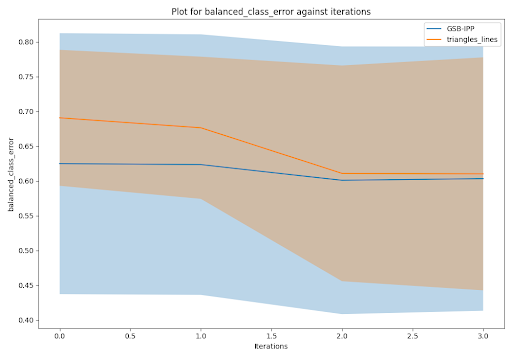
\includegraphics[width=0.45\textwidth]{figs/results/ipp/error (2).png}}
    \hfill
    \subfloat{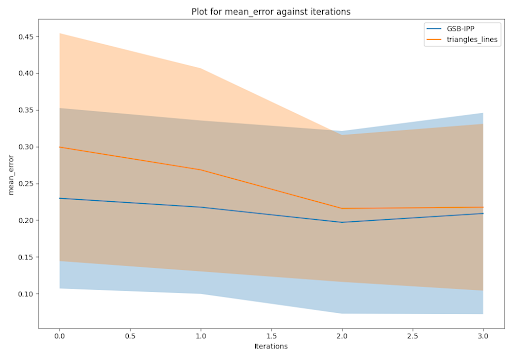
\includegraphics[width=0.45\textwidth]{figs/results/ipp/balanced_error (2).png}}
    \hfill
    \centering
    \subfloat{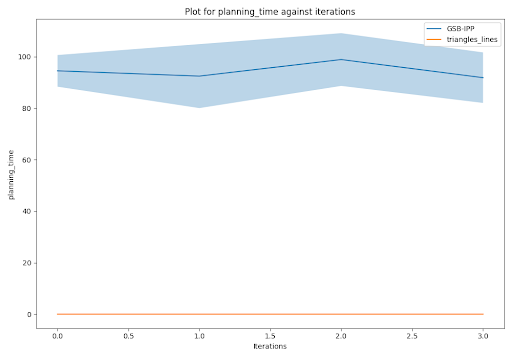
\includegraphics[width=0.45\textwidth]{figs/results/ipp/timing_result (1).png}}
    \caption{Quantitative statistics for the informative path planning approach.}
    \label{fig:results:ipp_quant}
\end{figure}



An interesting finding is that the performance of both approaches did not improve dramatically over the sampling iterations. This can likely be attributed to the simple prediction model we used which saturated quickly. The performance of the proposed planner was especially stable. This suggests that it was able to very quickly saturate the prediction model by choosing a representative set of samples in the first round.The performance would probably increase more over time if we used a more complex prediction system, instead of nearest neighbor. 

The timing results, seen in the leftmost part of Figure~\ref{fig:results:ipp_quant}, show that the algorithm can plan a mission in approximately 100 seconds using a laptop with a RTX3700 GPU. This shows that this approach is extremely feasible for deployment under operational constraints. An interesting finding is that the timing does not increase significantly over iterations. This is interesting because during the uncertainty estimation portion of the approach we use an increasingly-large Gaussian Process. We expected that the order $n^3$ time of this step would dominate the system runtime, but this was not the case. We will further profile the system timing in future work.


